\documentclass[main.tex]{subfiles}
\begin{document}
\chapter{Komplexe Zahlen}
\chapterauthor{Pascal}


\section{Einführung}

	Die Ursache für die Einführung der komplexen Zahlen ist vergleichbar mit der jeglicher anderer Zahlenmengen (abgesehen
	von $\N$). Alles basiert auf einer Rechnung oder einer Menge an Rechnungen, welche für die vorhandenen Zahlenmengen \textbf{keine Lösung besitzen} oder aber diese Zahlenmengen einem nicht erlauben eine Lösung zu finden. Ein Beispiel hierfür ist die Einführung der
	negativen Zahlen. Gleichungen der Form $2 + x = 1$ waren eine Zeit lang nicht lösbar. Ebenso galt einmal, dass $x^2 - 2 = 0$ keine
	Lösung besitzt, da hierfür die reellen Zahlen benötigt werden. Analog dazu wird die Erweiterung auf die komplexen Zahlen begründet.
	Dies wird an folgendem klassischen Beispiel erläutert:

	\begin{align*}
		\qquad \qquad x^2 + 1 &= 0 \\
			\Leftrightarrow x &= \sqrt{-1} \quad \text{\lightning}
	\end{align*}

	Um dieser und anderen Gleichungen eine Lösung zuzuteilen ist es nicht nur notwendig die Zahlenmenge zu erweitern, sondern
	auch, neue Symbole und Zeichen einzuführen um die neuen Zahlen zu kennzeichnen. Für die $\Z$ ist es das Symbol \dq-\dq, für $\Q$
	\dq,\dq und $\dfrac{a}{b}$, für $\R$ $\sqrt{a}$ und die Zeichen $\pi$ und $e$ zum Beispiel (auch wenn beide sich anders darstellen lassen). (Ein) gewisse(r) Mathematiker (Leibniz glaube ich) hat entschieden, dass das einzige benötigte Zeichen $i$ sein sollte, da er sie imaginäre Zahl nannte (Für den Fall, dass ich hier ein bisschen was durcheinander bringe, sind Direktverbesserungen kommentarlos erlaubt und erwünscht).

	\begin{Definition}[Imaginäre Einheit]
		Die Ikone $i$ der komplexen Zahl trägt den Namen \textbf{imaginäre Einheit} und wird folglich definiert:
		$$i \in \C : i^2 = -1; \C \:= \R \cup \left \{ i \right \}$$
	\end{Definition}

	\subsubsection{Algebraische Form}

	\begin{Definition}[Algebraische Formel]
		Komplexe Zahlen werden im Allgemeinen mit dem Buchstaben $z$ dargestellt oder aber auch $z_I$, wobei $I$ ein Punkt der Gauß'schen Zahlenebene ist (Weiteres hierzu folgt). Die sogenannte \textbf{algebraische / arithmetische Form} einer solchen Zahl wird wie folgt definiert:
		
		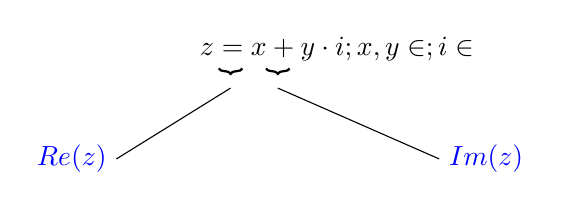
\begin{tikzpicture}
			%\draw (0,0) node {" "};
			\draw (7.9, 0) node {$z = x + y \cdot i; x,y \in \R; i \in \C$};
			\draw[line width=0.8pt][decorate,decoration={brace,amplitude=2pt},rotate around={180:(7.3,-0.25)}] (7.3,-0.25) -- (7.6,-0.25);
			\draw[line width=0.8pt][decorate,decoration={brace,amplitude=2pt},rotate around={180:(6.7,-0.25)}] (6.7,-0.25) -- (7,-0.25);
		    \draw[line width=0.4pt] (6.55,-0.5) -- (5.1,-1.4) node[color=blue,left] {$Re(z)$};
		    \draw[line width=0.4pt] (7.15,-0.5) -- (9.2,-1.4) node[color=blue,right] {$Im(z)$};
		\end{tikzpicture}
		\\
		Hierbei wird $x = Re(z)$ \textbf{Realteil} und $y = Im(z)$ und zwar \textbf{nur $y$ Imaginärteil} genannt.
	\end{Definition}

	\begin{Bemerkung}
		Eine Zahl $z = x + yi \in \C$ heißt \textbf{rein imaginär} für $x = 0$.
		\\
		Analog dazu wird sie für $y = 0$ als reell bezeichnet.
	\end{Bemerkung}


\section{Der Körper der komplexen Zahlen}

	Da wir nun wissen (oder halt auch nicht), weshalb wir die komplexen Zahlen benötigen, gilt es nun die verschiedenen Verknüpfungen, mit welchen wir zwei komplexe Zahlen verbinden, zu definieren. Wie alle anderen bekannten Mengen (außer $\N$), ist $\C$ teil eines \textbf{Körpers} welcher die zwei Verknüpfungen, denen wir allgemein die Namen \textbf{Addition} und \textbf{Multiplikation} geben. Das 3-Tupel (oder auch Tripel) ($\C$, +, *) ist somit der Körper, mit welchem wir arbeiten werden (jemals gefragt warum keine weiteren Verknüpfungen eingeführt wurden?). Jedoch muss auch erstmal bewiesen werden, dass dieses Tripel ein Körper ist:

	\begin{Beweis}
		\underline{\textbf{Die Addition}}:

		Für die Addition gilt bekanntlich zu beweisen, dass ($\C$, $\oplus$) eine abelsche oder auch kommutative Gruppe ist:

		\begin{enumerate}
			\item \begin{align*}
						\forall z_1, z_2 \in \C: z_1 \oplus z_2 &\:= (x_1 + y_1i) \oplus (x_2 + y_2i) \\
														   		&= ((x_1 + x_2) + (y_1 + y_2)i) \\
														   		&\in \C \\
						\Rightarrow \forall z_1, z_2 \in \C: \oplus : \C \times \C \rightarrow \C & \quad \text{(Abgeschlossenheit)}
				  \end{align*}
			\item \begin{align*}
				  		(z_1 \oplus z_2) \oplus z_3 &= ((x_1 + x_2) + (y_1 + y_2)i) \oplus (x_3 + y_3i) \\
										  			&= ((x_1 + x_2 + x_3) + (y_1 + y_2 + y_3)i) \\
												    &= (x_1 + y_1i) \oplus ((x_2 + x_3) + (y_2 + y_3)i) \\
												    &= (x_1 + y_1i) \oplus ((x_2 + y_2i) \oplus (x_3 + y_3i)) \\
												    &= z_1 \oplus (z_2 \oplus z_3) \\
						\Rightarrow \forall z_1, z_2, z_3 \in \C: (z_1 + &z_2) \oplus  z_3 = z_1 \oplus (z_2 + z_3) \quad \text{(Assoziativität)}
				  \end{align*}
			\item \begin{align*}
						0 = (0 + 0i) \in \C, \forall z \in \C:& \\
												   z \oplus 0 &= (x + yi) \oplus (0 + 0i) \\
													  		  &= ((x + 0) + (y + 0)i) \\
															  &= (x + yi) \\
															  &= z \\
						\Rightarrow \exists! 0: z \oplus 0 = z; z \in \C \quad &\text{(Neutrales Element)}
				  \end{align*}
			\item \begin{align*}
	  					-z = -(x + yi) \in \C, z \in \C &: \\
								  z \oplus (-z) =& (x + yi) \oplus (-(x + yi)) \\
								  			  =& ((x - x) + (y - y)i) \\
											  =& (0 + 0i) \\
											  =& 0  \\
						\Rightarrow \forall z \in \C \exists -z: z \oplus -z = 0 \quad \text{(Inverses Element)} \qquad &
	  			  \end{align*}
			\item \begin{align*}
						z_1 \oplus z_2 &= (x_1 + y_1i) \oplus (x_2 + y_2i) \\
									   &= ((x_1 + x_2) + (y_1 + y_2)i) \\
									   &= ((x_2 + x_1) + (y_2 + y_1)i) \\
									   &= (x_2 + y_2i) \oplus (x_1 + y_1i) \\
									   &= z_2 \oplus z_1 \\
						\Rightarrow \forall z_1, z_2 \in \C: z_1 \oplus z_2 = z_2 \oplus z_1 \quad \text{(Kom}&\text{mutativität)}
				  \end{align*}
		\end{enumerate}
		\newpage
		\underline{\textbf{Die Multiplikation}}:

		Für die Multiplikation gilt ebenfalls zu beweisen, dass ($\C$, $\otimes$) eine kommutative Gruppe ist:

		\begin{enumerate}
			\item \begin{align*}
						\forall z_1, z_2 \in \C: z_1 \otimes z_2 &\:= (x_1 + y_1i) \otimes (x_2 + y_2i) \\
														   		 &= ((x_1x_2 - y_1y_2) + (x_1y_2 + x_2y_1)i) \\
														   		 &\in \C \\
						\Rightarrow \forall z_1, z_2 \in \C: \otimes : \C \times \C \rightarrow \C & \quad \text{(Abgeschlossenheit)}
				  \end{align*}
			\item \begin{align*}
				  		(z_1 \otimes z_2) \otimes z_3 &= ((x_1x_2 - y_1y_2) + (x_1y_2 + x_2y_1)i) \otimes (x_3 + y_3i) \\
										  			  &= ((x_1x_2x_3 - y_1y_2x_3 - x_1y_2y_3 - x_2y_1y_3) + (x_1x_2y_3 - y_1y_2y_3 + x_1y_2x_3 + x_2y_1x_3)i) \\
												      &= (x_1 + y_1i) \otimes ((x_2x_3 - y_2y_3) + (x_2y_3 + x_3y_2)i) \\
												      &= (x_1 + y_1i) \otimes ((x_2 + y_2i) \otimes (x_3 + y_3i)) \\
												      &= z_1 \otimes (z_2 \otimes z_3) \\
						\Rightarrow \forall z_1, z_2, z_3 \in \C: (z_1 + &z_2) \otimes  z_3 = z_1 \otimes (z_2 + z_3) \quad \text{(Assoziativität)}
				  \end{align*}
			\item \begin{align*}
						1 = (1 + 0i) \in \C, \forall z \in \C:& \\
												   z \otimes 1 &= (x + yi) \otimes (1 + 0i) \\
													  		   &= ((1 \cdot x - 0 \cdot y) + (1 \cdot y + 0 \cdot x)i) \\
															   &= (x + yi) \\
															   &= z \\
						\Rightarrow \exists! 1: z \otimes 1 = z; z \in \C \quad &\text{(Neutrales Element)}
				  \end{align*}
			\item \begin{align*}
	  					z^{-1} = (x + yi)^{-1} \in \C, z \in \C:& \\
								  z \otimes z^{-1} &= (x + yi) \otimes \dfrac{1}{(x + yi)} \\
								  			  	   &= \dfrac{(x + yi) \cdot (x - yi)}{(x + yi) \cdot (x - yi)} \\
												   &= \dfrac{((x^2 + y^2) + (0i))}{((x^2 + y^2) + (0i))} \\
											  	   &= (1 + 0i) \\
											  	   &= e \\
						\Rightarrow \forall z \in \C \exists z^{-1}: z \otimes z^{-1} = 1 \quad \text{(Inverses Element)} \qquad &
	  			  \end{align*}
			\item \begin{align*}
						z_1 \otimes z_2 &= (x_1 + y_1i) \otimes (x_2 + y_2i) \\
									    &= ((x_1x_2 - y_1y_2) + (x_1y_2 + x_2y_1)i) \\
									    &= ((- y_1y_2 + x_1x_2) + (x_2y_1 + x_1y_2)i) \\
									    &= (x_2 + y_2i) \otimes (x_1 + y_1i) \\
									    &= z_2 \otimes z_1 \\
						\Rightarrow \forall z_1, z_2 \in \C: z_1 \otimes z_2 = z_2 \otimes z_1 \quad \text{(Kom}&\text{mutativität)}
				  \end{align*}
		\end{enumerate}
		\newpage
		\underline{\textbf{Auch Verknüpfungen sind Gesellschaftswesen, gemeinsam glänzen sie}}:
		Zu guter Letzt muss das Distributivgesetz gelten: (Bidde schön Frau Rämie mol)
			\begin{align*}
				(z_1 \oplus z_2) \otimes z_3 &= ((x_1 + y_1i) \oplus (x_2 + y_2i)) \otimes (x_3 + y_3i) \\
											 &= ((x_1 + x_2) +  (y_1 + y_2)i) \otimes (x_3 + y_3i) \\
											 &= ((x_1x_3 + x_2x_3 - y_1y_3 - y_2y_3) + (x_1y_3 + x_2y_3 + y_1x_3 + y_2x_3)i) \\
											 &= ((x_1x_3 - y_1y_3) + (x_1y_3 + x_3y_1)i) + ((x_2x_3 - y_2y_3) + (x_2y_3 + x_3y_2)i) \\
											 &= (x_1 + y_1i) \otimes (x_3 + y_3i) \oplus (x_2 + y_2i) \otimes (x_3 + y_3i) \\
											 &= z_1 \otimes z_3 \oplus z_2 \otimes z_3 \\
			\Rightarrow \forall z_1, z_2, z_3 \in \C: (z_1 &\oplus z_2) \otimes z_3 = z_1 \otimes z_3 \oplus z_2 \otimes z_3 \quad \text{(Distributivität)}
			\end{align*}
	\end{Beweis}


\section{Die Gauß'sche Zahlenebene}

	\subsection{Einleitung}

		\subsubsection{Hinführung}

		Der Körper der komplexen Zahlen wurde nun definiert, wohingegen der Platz dieser auf unserem allbekannten Zahlensystem schleierhaft bleibt.
		Um einen Ansatz für eine Integration zu finden, bietet sich an zu beobachten, wie sich komplexe Zahlen auf der \textbf{reellen Zahlengerade} (welche eine Veranschaulichung des euklidischen Vektorraums $\R^1$ ist) verhalten.
		\\
		\begin{Definition}
			Als \textbf{Zeiger} wird ein visuelles Hilfsmittel definiert, welches in der Gauß'schen Zahlenebene das Analoge zu dem Pfeil eines Ortsvektors eines Vektorraumes ist.
		\end{Definition}

		\begin{center}
			\begin{tikzpicture}[>=triangle 45]
				\draw[->,line width=0.8pt] (-5.5,0) -- (6,0) node[above] {$Re(z)$};
				\foreach  \x in {-5,...,5}
	    			\draw (\x,0.2) -- (\x,-0.2) node[below] {$\x$};
				\draw[->,line width=0.8pt,color=red] (0,0) -- (3,0);
			\end{tikzpicture}
		\end{center}

		Addition und Multiplikation mit einem positiven Faktor im $\R^1$ sind nicht von Interesse, wohingegen die Multiplikation mit einem negativen Faktor uns reichlich mehr mitteilt:

		\begin{center}
			\begin{tikzpicture}[>=triangle 45]
				\draw[->,line width=0.8pt] (-5.5,0) -- (6,0) node[above] {$Re(z)$};
				\foreach  \x in {-5,...,5}
	    			\draw (\x,0.2) -- (\x,-0.2) node[below] {$\x$};
				\draw[->,line width=1.5pt,color=red] (0,0) -- (-3,0);
				\draw[->,line width=1.5pt,color=orange] (0,0) -- (4,0);
				\draw[->,line width=1.5pt,color=red,dashed] (0,0) -- (3,0);
				\draw[->,line width=1.5pt,color=orange,dashed] (0,0) -- (2,0);
				\draw[line width=1.3pt,color=red] (1.5,0.4) node {3};
				\draw[line width=1.3pt,color=red] (-1.5,0.4) node {-3};
				\draw[->,color=red] (2.4,0) arc (0:180:2.4);
				\draw[line width=2pt,color=white] (1.84,1.54) arc (40:55:2.4);
				\draw[->,color=orange] (0.3,0) arc (180:0:1.5);
				\draw[line width=0.8pt,color=orange] (1.8,1.8) node {$\cdot(2) = $ Skalierung mit Faktor $2$};
				\draw[line width=0.8pt,color=red] (0,2.7) node {$\cdot (-1) = 180°$ Drehung};
			\end{tikzpicture}
		\end{center}

		Da gilt, dass: $i^2 = -1$ ist die Multiplikation einer reellen Zahl mit $i^2$ äquivalent zu einer $180$ - Grad Drehung. Daraus lässt sich schließen, dass die Multiplikation mit $i$ einer \textbf{$90$ - Grad Drehung} entspricht, da: $a \cdot i^2 = a \cdot i \cdot i; a\in\R$ und man davon ausgeht, dass $\cdot(i)$ bei jeder Instanz dieselbe Transformation anwendet. Somit entsteht eine wunderschöne Ebene, in der alle Zahlen zusammen spielen und sich amüsieren können:
		
		\begin{center}
			\begin{tikzpicture}[>=triangle 45]
				\draw[->,line width=0.8pt] (-5.5,0) -- (5.7,0) node[above] {$Re(z)$};
				\draw[->,line width=0.8pt] (0,-5.5) -- (0,5.7) node[right] {$Im(z)$};
				\foreach  \x in {-5,...,-1,1,2,...,5}
	                \draw [line width=0.8pt] (\x,0.1) -- (\x,-0.1) node[below] {$\x$};
	            \foreach  \x in {-5,...,-1,1,2,...,5}
	                \draw [line width=0.8pt] (-0.1,\x) -- (0.1,\x) node[right] {$\x i$};
				\draw[line width=0.8pt] (-0.2,-0.2) node {$O$};
				\draw[->,line width=1.5pt,color=red] (0,0) -- (-3,0);
				\draw[->,line width=1.5pt,color=red,dashed] (0,0) -- (3,0);
				\draw[line width=1.3pt,color=red] (1.5,0.3) node {3};
				\draw[line width=1.3pt,color=red] (-1.5,0.3) node {-3};
				\draw[->,line width=1.5pt,color=red] (0,0) -- (0,-3);
				\draw[->,line width=1.5pt,color=red] (0,0) -- (0,3);
				\draw[line width=1.3pt,color=red] (-0.3,1.5) node {$3i$};
				\draw[line width=1.3pt,color=red] (-0.4,-1.5) node {$-3i$};
				\draw[->,color=red] (2.4,0) arc (0:90:2.4);
				\draw[->,color=red] (0,2.4) arc (90:180:2.4);
				\draw[line width=1.3pt,color=red] (1.9,2) node {$\cdot(i)$};
				\draw[line width=1.3pt,color=red] (-1.9,2) node {$\cdot(i)$};
				\draw[->,color=red] (2.4,0) arc (360:270:2.4);
				\draw[->,color=red] (0,-2.4) arc (270:180:2.4);
				\draw[line width=1.3pt,color=red] (1.9,-2) node {$\cdot(-i)$};
				\draw[line width=1.3pt,color=red] (-1.9,-2) node {$\cdot(-i)$};
			\end{tikzpicture}
		\end{center}

		\begin{Definition}[Gauß'sche Zahlenebene]
			Seien eine reelle Achse mit Einheit 1 und eine imaginäre Achse mit Einheit $i$. Dann nennt sich \textbf{Gauß'sche Zahlenebene} gerade die Ebene, welche als Achsen die zueinander orthogonalen genannten Achsen hat. Konvention ist es, die imaginäre Achse vertikal zu platzieren.
			\begin{center}
				\begin{tikzpicture}[>=triangle 45]
					\draw [step=1cm,lightgray,very thin] (-4.9,-4.9) grid (4.9,4.9);
					\draw[->,line width=0.8pt] (-5.5,0) -- (5.7,0) node[above] {$Re(z)$};
					\draw[->,line width=0.8pt] (0,-5.5) -- (0,5.7) node[right] {$Im(z)$};
					\foreach  \x in {-5,...,-1,1,2,...,5}
		                \draw [line width=0.8pt] (\x,0.1) -- (\x,-0.1) node[below] {$\x$};
		            \foreach  \x in {-5,...,-2,2,3,...,5}
		                \draw [line width=0.8pt] (-0.1,\x) -- (0.1,\x) node[right] {$\x i$};
					\draw[line width=0.8pt] (-0.1,1) -- (0.1,1) node[right] {$i$};
					\draw[line width=0.8pt] (-0.1,-1) -- (0.1,-1) node[right] {$-i$};
					\draw[line width=0.8pt] (-0.2,-0.2) node {$O$};
					\draw[->,line width=1.5pt,color=red,dashed] (0,0) -- (2,0);
					\draw[->,line width=1.5pt,color=red,dashed] (2,0) -- (2,3);
					\draw[->,line width=1.5pt,color=red] (0,0) -- (2,3);
					\draw[line width=1.3pt,color=red] (1,0.3) node {$2$};
					\draw[line width=1.3pt,color=red] (1.65,0.9) node {$+$};
					\draw[line width=1.3pt,color=red] (2.3,1.5) node {$3i$};
					\draw[line width=1.3pt,color=red] (0.85,2.35) node {$2 + 3i$};
					\draw[line width=0.8pt] (2.25,3.25) node {$A$};
					\draw[line width=0.8pt,fill=black] (2,3) circle (1.5pt);
				\end{tikzpicture}
			\end{center}
		\end{Definition}

		\begin{Bemerkung}
			Da jede komplexe Zahl eine Darstellung in der Gauß'schen Zahlenebene besitzt, lassen sie sich ebenfalls über einen Winkel und den Abstand zum Origo beschreiben.
		\end{Bemerkung}

		\begin{Definition}[Betrag einer komplexen Zahl]
			Der \textbf{Betrag} einer komplexen Zahl ist gleichbedeutend mit dem \textbf{Abstand der Zahl zum Origo} oder der Länge des Zeigers. Pythagoras liefert uns eine Formel:
			$$|z| := \sqrt{x^2 + y^2} ; z = x + yi$$
		\end{Definition}

		\begin{Definition}[Argument einer komplexen Zahl]
			Das \textbf{Argument} einer komplexen Zahl ist gleichbedeutend mit dem \textbf{Winkel der Zahl}, welcher der Zeiger mit der \glqq rechten Hälfte\grqq der reellen Achse einschließt (im mathematischen Sinn und modulo $2\pi$). Pythagoras liefert uns weitere Formeln:

			\begin{enumerate}
				\item 1. und 3. Quadrant: $$arg(z) \:= \tan^{-1}\left(\dfrac{y}{x}\right) + \dfrac{\pi}{2} \cdot (\text{Quadrant} - 1) ; z = x + yi$$
				\item 2. und 4. Quadrant: $$arg(z) = \tan^{-1}\left(\dfrac{x}{y}\right) + \dfrac{\pi}{2} \cdot (\text{Quadrant} - 1) ; z = x + yi$$
			\end{enumerate}

		\end{Definition}

		\begin{Definition}[Betrag-Winkel Form]
			Als \textbf{Betrag-Winkel Form} wird eine Darstellungsform einer komplexen Zahl definiert, welche diese explizit über deren Argument und Betrag definiert. Sie ist keine offizielle Darstellungsweise einer komplexen Zahl, jedoch bringt sie uns der nächsten wichtigen näher und fasst die zwei vorangehenden Definitionen zusammen.
													$$z = |z|_{arg(z)}; z \in \C$$
		\end{Definition}

	\subsection{Polarform}

		\begin{Definition}[Polarform]
			Die \textbf{Polarform} einer komplexen Zahl definiert diese Zahl (wie auch die Betrag-Winkel Form) über deren \textbf{Argument und Betrag}.
													$$z = |z| \cdot (\cos(arg(z)) + \sin(arg(z))i)$$
		\end{Definition}

		\begin{Beweis}
			Nach dem Satz von Pythagoras gilt $\forall z = x + yi ; z \in \C$:
			\\\\
			\begin{minipage}{0.29\textwidth}
				\text{ }
			\end{minipage}
			\begin{minipage}{0.71\textwidth}
				$$\Rightarrow	 \begin{vmatrix}
					\dfrac{x}{|z|} &= \cos(arg(z)) 	   \\
					\dfrac{y}{|z|} &= \sin(arg(z)) 	   \\
								|z| &= \sqrt{x^2 + y^2} \\
				\end{vmatrix}$$
				$$\Leftrightarrow \begin{vmatrix}
						x &= \cos(arg(z)) \cdot |z| \\
						y &= \sin(arg(z)) \cdot |z| \\
					|z| &= \sqrt{x^2 + y^2} 	  \\
				\end{vmatrix}$$
			\end{minipage}
			\\\\
			\abovedisplayskip=-\baselineskip
			\belowdisplayskip=0pt
			\abovedisplayshortskip=-\baselineskip
			\belowdisplayshortskip=0pt
			\begin{align*}
				\Rightarrow z &= x + yi \\
							  &= \cos(arg(z)) \cdot |z| + (\sin(arg(z)) \cdot |z|)i \\
							  &= |z| \cdot (\cos(arg(z)) + \sin(arg(z))i)
			\end{align*}

		\end{Beweis}

	\subsection{Rechenoperationen in der Gauß'schen Zahlenebene}

		Die bereits angesprochenen basischen Rechenoperationen lassen sich in der Gauß'schen Zahlenebene als Transformation darstellen. Weshalb dies interessant ist, wird im Verlauf dieses Abschniits hoffentlich noch deutlich.
		Die Addition ist die einfachste Transformation, weil sie equivalent zur Linearkombination bei Vektoren ist, da gilt: $$(z_1 + z_2) = ((x_1 + x_2) + (y_1 + y_2)i)$$ Bildlich bedeutet das:

		\begin{center}
			\begin{tikzpicture}[>=triangle 45]
				\draw[->,line width=0.8pt] (-5.5,0) -- (5.7,0) node[above] {$Re(z)$};
				\draw[->,line width=0.8pt] (0,-5.5) -- (0,5.7) node[right] {$Im(z)$};
				\foreach  \x in {-5,...,-1,1,2,...,5}
	                \draw [line width=0.8pt] (\x,0.1) -- (\x,-0.1) node[below] {$\x$};
	            \foreach  \x in {-5,...,-2,2,3,...,5}
	                \draw [line width=0.8pt] (-0.1,\x) -- (0.1,\x) node[right] {$\x i$};
				\draw[line width=0.8pt] (-0.1,1) -- (0.1,1) node[right] {$i$};
				\draw[line width=0.8pt] (-0.1,-1) -- (0.1,-1) node[right] {$-i$};
				\draw[line width=0.8pt] (-0.2,-0.2) node {$O$};
				\draw[->,line width=1.5pt,color=black,dashed] (0,0) -- (5,0);
				\draw[->,line width=1.5pt,color=black,dashed] (5,0) -- (5,4);
				\draw[->,line width=1.5pt,color=orange,dashed] (0,0) -- (3,0);
				\draw[->,line width=1.5pt,color=red,dashed] (0,0) -- (2,0);
				\draw[->,line width=1.5pt,color=red,dashed] (2,0) -- (2,3);
				\draw[->,line width=1.5pt,color=orange,dashed] (3,0) -- (3,1);
				\draw[->,line width=1.5pt,color=red] (0,0) -- (2,3);
				\draw[->,line width=1.5pt,color=orange] (0,0) -- (3,1);
				\draw[->,line width=1.5pt,color=black] (0,0) -- (5,4);
				\draw[line width=1.3pt,color=red] (1.5,0.3) node {$2$};
				\draw[line width=1.3pt,color=red] (2.3,1.5) node {$3i$};
				\draw[line width=1.3pt,color=red] (2.2,3.2) node {$2 + 3i$};
				\draw[line width=1.3pt,color=orange] (2.3,0.3) node {$3$};
				\draw[line width=1.3pt,color=orange] (3.3,0.5) node {$i$};
				\draw[line width=1.3pt,color=orange] (3.2,1.2) node {$3 + i$};
				\draw[line width=1.3pt,color=black] (4.2,0.3) node {$2 + 3 = 5$};
				\draw[line width=1.3pt,color=black] (6,2) node {$3i + i = 4i$};
				\draw[line width=1.3pt,color=black] (5.2,4.2) node {$5 + 4i$};
			\end{tikzpicture}
		\end{center}

		Im Gegensatz dazu ist die Multiplikation weniger intuitiv. Aus logistischen Gründen wird sie trotz allem in diesem Abschnitt besprochen. Bildlich stellt sie eine Drehstreckung dar (auch dies wird gegen Ende des Kapitels genauer beschrieben), da gilt:
		$$(z_1 \cdot z_2) = r_{1_{\alpha}} \cdot r_{2_{\beta}} = (r_1 \cdot r_2)_{\alpha + \beta}$$

		\begin{center}
			\begin{tikzpicture}[>=triangle 45]
				\draw[line width=0.8pt,color=black,fill=black,fill opacity=0.1] (0,0) -- (4,0) arc (0:135:4) -- cycle;
				\draw[line width=0.8pt,color=orange,fill=orange,fill opacity=0.3] (0,0) -- (1.2,0) arc (0:116.565:1.2) -- cycle;
				\draw[line width=0.8pt,color=red,fill=red,fill opacity=0.3] (0,0) -- (2,0) arc (0:18.435:2) -- cycle;
				\draw[->,line width=0.8pt] (-5.5,0) -- (5.7,0) node[above] {$Re(z)$};
				\draw[->,line width=0.8pt] (0,-5.5) -- (0,5.7) node[right] {$Im(z)$};
				\foreach  \x in {-5,...,-1,1,2,...,5}
	                \draw [line width=0.8pt] (\x,0.1) -- (\x,-0.1) node[below] {$\x$};
	            \foreach  \x in {-5,...,-2,2,3,...,5}
	                \draw [line width=0.8pt] (-0.1,\x) -- (0.1,\x) node[right] {$\x i$};
				\draw[line width=0.8pt] (-0.1,1) -- (0.1,1) node[right] {$i$};
				\draw[line width=0.8pt] (-0.1,-1) -- (0.1,-1) node[right] {$-i$};
				\draw[line width=0.8pt] (-0.2,-0.2) node {$O$};
				\draw[->,line width=1.5pt,color=red] (0,0) -- (3,1);
				\draw[->,line width=1.5pt,color=orange] (0,0) -- (-1,2);
				\draw[->,line width=1.5pt,color=black] (0,0) -- (-5,5);
				\draw[line width=1.3pt,color=red] (3.2,1.2) node {$3 + i$};
				\draw[line width=1.3pt,color=orange] (-1.2,2.2) node {$-1 + 2i$};
				\draw[line width=1.3pt,color=black] (-5.2,5.2) node {$-5 + 5i$};
				\draw[line width=0.8pt,color=red] (1.5,0.25) node {$\alpha$};
				\draw[line width=0.8pt,color=orange] (0.5,0.6) node {$\beta$};
				\draw[line width=0.8pt,color=black] (1.5,2) node {$\alpha + \beta$};
				\draw[line width=0.8pt,color=black] (-3.3,2.2) node {$r = r_1 \cdot r_2$};
			\end{tikzpicture}
		\end{center}
\end{document}
